% Options for packages loaded elsewhere
\PassOptionsToPackage{unicode}{hyperref}
\PassOptionsToPackage{hyphens}{url}
%
\documentclass[
  10pt,
  ignorenonframetext,
  aspectratio=169,handout]{beamer}
\usepackage{pgfpages}
\setbeamertemplate{caption}[numbered]
\setbeamertemplate{caption label separator}{: }
\setbeamercolor{caption name}{fg=normal text.fg}
\beamertemplatenavigationsymbolsempty
% Prevent slide breaks in the middle of a paragraph
\widowpenalties 1 10000
\raggedbottom
\setbeamertemplate{part page}{
  \centering
  \begin{beamercolorbox}[sep=16pt,center]{part title}
    \usebeamerfont{part title}\insertpart\par
  \end{beamercolorbox}
}
\setbeamertemplate{section page}{
  \centering
  \begin{beamercolorbox}[sep=12pt,center]{section title}
    \usebeamerfont{section title}\insertsection\par
  \end{beamercolorbox}
}
\setbeamertemplate{subsection page}{
  \centering
  \begin{beamercolorbox}[sep=8pt,center]{subsection title}
    \usebeamerfont{subsection title}\insertsubsection\par
  \end{beamercolorbox}
}
\AtBeginPart{
  \frame{\partpage}
}
\AtBeginSection{
  \ifbibliography
  \else
    \frame{\sectionpage}
  \fi
}
\AtBeginSubsection{
  \frame{\subsectionpage}
}
\usepackage{amsmath,amssymb}
\usepackage{iftex}
\ifPDFTeX
  \usepackage[T1]{fontenc}
  \usepackage[utf8]{inputenc}
  \usepackage{textcomp} % provide euro and other symbols
\else % if luatex or xetex
  \usepackage{unicode-math} % this also loads fontspec
  \defaultfontfeatures{Scale=MatchLowercase}
  \defaultfontfeatures[\rmfamily]{Ligatures=TeX,Scale=1}
\fi
\usepackage{lmodern}
\usetheme[]{Boadilla}
\usecolortheme{orchid}
\usefonttheme{structurebold}
\useinnertheme{rounded}
\ifPDFTeX\else
  % xetex/luatex font selection
\fi
% Use upquote if available, for straight quotes in verbatim environments
\IfFileExists{upquote.sty}{\usepackage{upquote}}{}
\IfFileExists{microtype.sty}{% use microtype if available
  \usepackage[]{microtype}
  \UseMicrotypeSet[protrusion]{basicmath} % disable protrusion for tt fonts
}{}
\makeatletter
\@ifundefined{KOMAClassName}{% if non-KOMA class
  \IfFileExists{parskip.sty}{%
    \usepackage{parskip}
  }{% else
    \setlength{\parindent}{0pt}
    \setlength{\parskip}{6pt plus 2pt minus 1pt}}
}{% if KOMA class
  \KOMAoptions{parskip=half}}
\makeatother
\usepackage{xcolor}
\newif\ifbibliography
\usepackage{color}
\usepackage{fancyvrb}
\newcommand{\VerbBar}{|}
\newcommand{\VERB}{\Verb[commandchars=\\\{\}]}
\DefineVerbatimEnvironment{Highlighting}{Verbatim}{commandchars=\\\{\}}
% Add ',fontsize=\small' for more characters per line
\usepackage{framed}
\definecolor{shadecolor}{RGB}{48,48,48}
\newenvironment{Shaded}{\begin{snugshade}}{\end{snugshade}}
\newcommand{\AlertTok}[1]{\textcolor[rgb]{1.00,0.81,0.69}{#1}}
\newcommand{\AnnotationTok}[1]{\textcolor[rgb]{0.50,0.62,0.50}{\textbf{#1}}}
\newcommand{\AttributeTok}[1]{\textcolor[rgb]{0.80,0.80,0.80}{#1}}
\newcommand{\BaseNTok}[1]{\textcolor[rgb]{0.86,0.64,0.64}{#1}}
\newcommand{\BuiltInTok}[1]{\textcolor[rgb]{0.80,0.80,0.80}{#1}}
\newcommand{\CharTok}[1]{\textcolor[rgb]{0.86,0.64,0.64}{#1}}
\newcommand{\CommentTok}[1]{\textcolor[rgb]{0.50,0.62,0.50}{#1}}
\newcommand{\CommentVarTok}[1]{\textcolor[rgb]{0.50,0.62,0.50}{\textbf{#1}}}
\newcommand{\ConstantTok}[1]{\textcolor[rgb]{0.86,0.64,0.64}{\textbf{#1}}}
\newcommand{\ControlFlowTok}[1]{\textcolor[rgb]{0.94,0.87,0.69}{#1}}
\newcommand{\DataTypeTok}[1]{\textcolor[rgb]{0.87,0.87,0.75}{#1}}
\newcommand{\DecValTok}[1]{\textcolor[rgb]{0.86,0.86,0.80}{#1}}
\newcommand{\DocumentationTok}[1]{\textcolor[rgb]{0.50,0.62,0.50}{#1}}
\newcommand{\ErrorTok}[1]{\textcolor[rgb]{0.76,0.75,0.62}{#1}}
\newcommand{\ExtensionTok}[1]{\textcolor[rgb]{0.80,0.80,0.80}{#1}}
\newcommand{\FloatTok}[1]{\textcolor[rgb]{0.75,0.75,0.82}{#1}}
\newcommand{\FunctionTok}[1]{\textcolor[rgb]{0.94,0.94,0.56}{#1}}
\newcommand{\ImportTok}[1]{\textcolor[rgb]{0.80,0.80,0.80}{#1}}
\newcommand{\InformationTok}[1]{\textcolor[rgb]{0.50,0.62,0.50}{\textbf{#1}}}
\newcommand{\KeywordTok}[1]{\textcolor[rgb]{0.94,0.87,0.69}{#1}}
\newcommand{\NormalTok}[1]{\textcolor[rgb]{0.80,0.80,0.80}{#1}}
\newcommand{\OperatorTok}[1]{\textcolor[rgb]{0.94,0.94,0.82}{#1}}
\newcommand{\OtherTok}[1]{\textcolor[rgb]{0.94,0.94,0.56}{#1}}
\newcommand{\PreprocessorTok}[1]{\textcolor[rgb]{1.00,0.81,0.69}{\textbf{#1}}}
\newcommand{\RegionMarkerTok}[1]{\textcolor[rgb]{0.80,0.80,0.80}{#1}}
\newcommand{\SpecialCharTok}[1]{\textcolor[rgb]{0.86,0.64,0.64}{#1}}
\newcommand{\SpecialStringTok}[1]{\textcolor[rgb]{0.80,0.58,0.58}{#1}}
\newcommand{\StringTok}[1]{\textcolor[rgb]{0.80,0.58,0.58}{#1}}
\newcommand{\VariableTok}[1]{\textcolor[rgb]{0.80,0.80,0.80}{#1}}
\newcommand{\VerbatimStringTok}[1]{\textcolor[rgb]{0.80,0.58,0.58}{#1}}
\newcommand{\WarningTok}[1]{\textcolor[rgb]{0.50,0.62,0.50}{\textbf{#1}}}
\usepackage{graphicx}
\makeatletter
\newsavebox\pandoc@box
\newcommand*\pandocbounded[1]{% scales image to fit in text height/width
  \sbox\pandoc@box{#1}%
  \Gscale@div\@tempa{\textheight}{\dimexpr\ht\pandoc@box+\dp\pandoc@box\relax}%
  \Gscale@div\@tempb{\linewidth}{\wd\pandoc@box}%
  \ifdim\@tempb\p@<\@tempa\p@\let\@tempa\@tempb\fi% select the smaller of both
  \ifdim\@tempa\p@<\p@\scalebox{\@tempa}{\usebox\pandoc@box}%
  \else\usebox{\pandoc@box}%
  \fi%
}
% Set default figure placement to htbp
\def\fps@figure{htbp}
\makeatother
\ifLuaTeX
  \usepackage{luacolor}
  \usepackage[soul]{lua-ul}
\else
  \usepackage{soul}
  \makeatletter
  \let\HL\hl
  \renewcommand\hl{% fix for beamer highlighting
    \let\set@color\beamerorig@set@color
    \let\reset@color\beamerorig@reset@color
    \HL}
  \makeatother
\fi
\setlength{\emergencystretch}{3em} % prevent overfull lines
\providecommand{\tightlist}{%
  \setlength{\itemsep}{0pt}\setlength{\parskip}{0pt}}
\setcounter{secnumdepth}{-\maxdimen} % remove section numbering
\newcommand{\setfigheight}[1]{\setkeys{Gin}{height=#1,keepaspectratio}}
\newcommand{\setfigwidth}[1]{\setkeys{Gin}{width=#1,keepaspectratio}}
\newcommand{\setrelfigwidth}[1]{\setfigwidth{#1\csname textwidth\endcsname}}
\newcommand{\setrelfigheight}[1]{\setfigheight{#1\csname textheight\endcsname}}
\usepackage{tikz}
\usetikzlibrary{arrows.meta}
theme/style.tex
\usepackage{bookmark}
\IfFileExists{xurl.sty}{\usepackage{xurl}}{} % add URL line breaks if available
\urlstyle{same}
\hypersetup{
  pdftitle={Python on Trillium and Open OnDemand},
  pdfauthor={Ramses van Zon},
  hidelinks,
  pdfcreator={LaTeX via pandoc}}

\title{Python on Trillium and Open OnDemand}
\author{Ramses van Zon}
\date{October 27, 2025}

\begin{document}
\frame{\titlepage}

\begin{frame}{In this workshop\ldots{}}
\phantomsection\label{in-this-workshop}
\begin{itemize}
\item
  Why Python?
\item
  Why Supercomputers?
\item
  Access
\item
  Using Trillium
\item
  Installing packages
\item
  More about OnDemand
\end{itemize}
\end{frame}

\section{Why Python?}\label{why-python}

\begin{frame}{Python is great}
\phantomsection\label{python-is-great}
\begin{itemize}
\item
  Python is a high-level, interpreted language.

  \pause
\item
  Python is fairly easy to learn, very expressive, and, not surprisingly, very popular.

  \pause
\item
  Its greatness is in large part due to the available packages.

  \pause
\item
  And in its interactive computing paradigm (=\textgreater{} Jupyter Lab)

  \pause
\item
  Development in Python can be substantially easier (and thus faster) than when using compiled languages.

  \pause
\item
  But the interpreted and dynamic nature of Python is often at odds with ``high performance''.\\
  \textbf{Yes, Python itself is slow!}

  \pause
\item
  This matters a lot less when Python is the `driver' or `glue language' for optimized packages or programs, such as for AI and ML.
\end{itemize}
\end{frame}

\begin{frame}{Running example}
\phantomsection\label{running-example}
\begin{columns}[T]
\begin{column}{0.31\linewidth}\setlength{\parskip}{0.5\baselineskip}
\pandocbounded{
\includegraphics[keepaspectratio]{fashion-mnist-sprite.png}}
\end{column}

\begin{column}{0.62\linewidth}\setlength{\parskip}{0.5\baselineskip}
\pause

\begin{itemize}
\item
  We have a data set of images of fashion items,\\
  \footnotesize (``T-shirt/top'', ``Trouser'', ``Pullover'', ``Dress'', ``Coat'', ``Sandal'',``Shirt'', ``Sneaker'', ``Bag'', ``Ankle boot''):\\
  See: \alert{\url{https://github.com/zalandoresearch/fashion-mnist}} \normalsize    

  \pause
\item
  We want to train an artificial neural work on this data set so we could recognize items in other images.

  \pause
\item
  We'll use PyTorch for this task.
\end{itemize}

\pause

This use case was taken from a PyTorch tutorial:\\
\footnotesize \alert{\url{https://docs.pytorch.org/tutorials/beginner/basics/quickstart_tutorial.html}}

\pause

\normalsize

Although this example would be too small to warrant running on the Trillium supercomputer, it will demonstrate many aspects of running Python applications on such a system.
\end{column}
\end{columns}
\end{frame}

\section{Why use a supercomputer?}\label{why-use-a-supercomputer}

\begin{frame}{Why use a supercomputer?}
\phantomsection\label{why-use-a-supercomputer-1}
Your research project may need more resources than your laptop can provide.

\pause

This may be for several reasons:

\pause

\begin{enumerate}
\item
  Your research computations are too large to fit on your laptop.

  \pause
\item
  The computations are too slow.

  \pause
\item
  The computations are too plentiful.
\end{enumerate}

\pause

\begin{columns}[T]
\begin{column}{0.47\linewidth}\setlength{\parskip}{0.5\baselineskip}
So you go to one of the Alliance's `advanced research computing' clusters: like Nibi, Fir, Narval, Rorqual and Trillium.
\end{column}

\begin{column}{0.47\linewidth}\setlength{\parskip}{0.5\baselineskip}
\pandocbounded{
\includegraphics[keepaspectratio]{Alliance_logo_English.png}}
\end{column}
\end{columns}

\pause

Congratulations, you are now doing \alert{Advanced Research Computing}!
\end{frame}

\section{Advanced Research Computing}\label{advanced-research-computing}

\begin{frame}{A supercomputer is just like your laptop}
\phantomsection\label{a-supercomputer-is-just-like-your-laptop}
\pause

Haha! You didn't really think so, right?\vspace{-1mm}

\begin{columns}[T]
\begin{column}{0.23\linewidth}\setlength{\parskip}{0.5\baselineskip}
\vspace{\baselineskip} \vspace{\baselineskip} \setkeys{Gin}{width=0.8\csname textwidth\endcsname,keepaspectratio} \centerline{\pandocbounded{
\includegraphics[keepaspectratio]{laptop.jpg}}} \vspace{\baselineskip} \vspace{\baselineskip} \only<3>{ We are going to need to make some adjustments. }
\end{column}

\begin{column}{0.69\linewidth}\setlength{\parskip}{0.5\baselineskip}
\pandocbounded{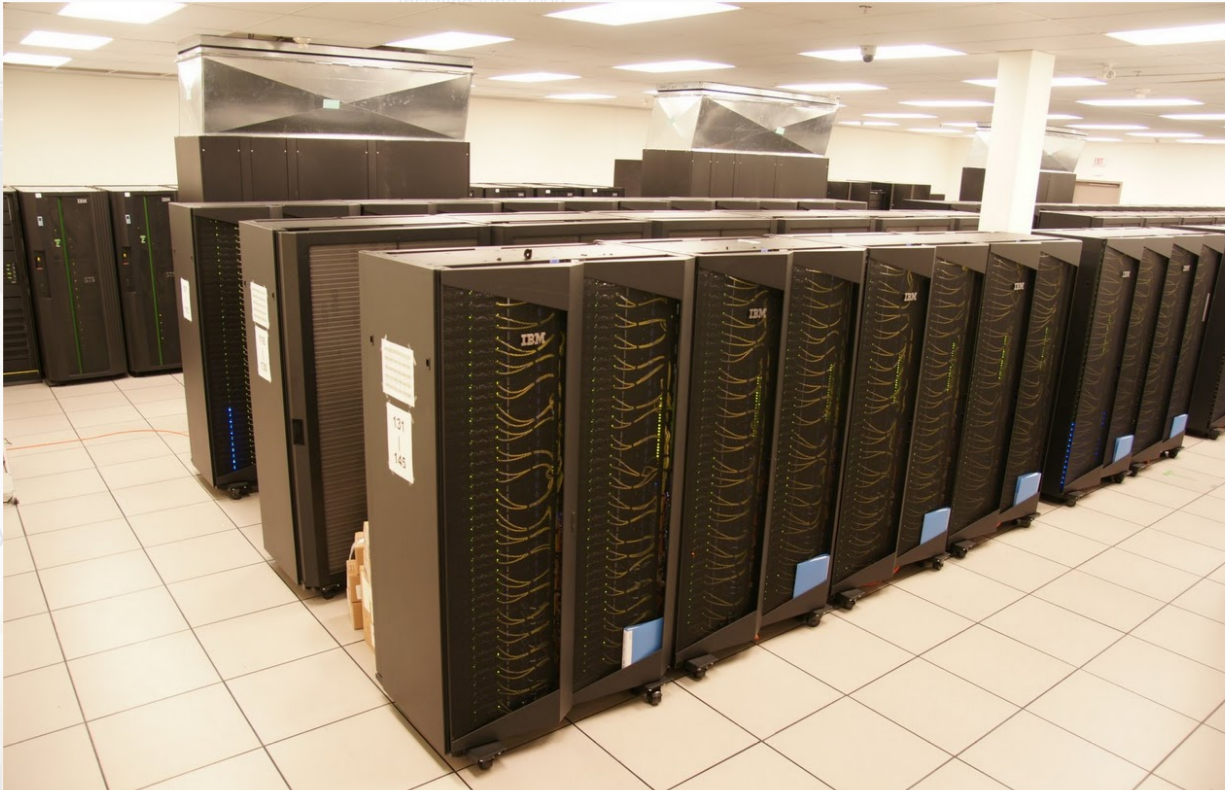
\includegraphics[keepaspectratio]{gpc.png}}
\end{column}
\end{columns}

\pause
\end{frame}

\begin{frame}{Using a supercomputer is different}
\phantomsection\label{using-a-supercomputer-is-different}
\pause

\begin{enumerate}
\item
  It is remote.

  \pause
\item
  It's usually command-line driven.

  \pause
\item
  It is a shared resource.

  \pause
\item
  It is not your own machine.
\end{enumerate}
\end{frame}

\begin{frame}{But it's still got Python, right?}
\phantomsection\label{but-its-still-got-python-right}
Well yes, but:

\pause

\begin{block}{}\setlength{\parskip}{0.5\baselineskip}
\phantomsection\label{section}
Many tutorials on Python, AI and ML assume that you are working on your own machine and have full privileges to reconfigure it (and mess it up). \vspace{\baselineskip}

\pause
\end{block}

\begin{block}{}\setlength{\parskip}{0.5\baselineskip}
\phantomsection\label{section-1}
We'll show you how to operate in this shared space, focusing in particular on Trillium\\
(but touching upon the other national systems as well). \vspace{\baselineskip}

\pause
\end{block}

\begin{block}{When do we get to running Jupyter notebooks?}\setlength{\parskip}{0.5\baselineskip}
\phantomsection\label{when-do-we-get-to-running-jupyter-notebooks}
\pause

Patience, we'll get there. \vspace{\baselineskip}
\end{block}
\end{frame}

\section{Getting started}\label{getting-started}

\begin{frame}{Let's get onto Trillium!}
\phantomsection\label{lets-get-onto-trillium}
What do you need to follow along this afternoon:

\begin{itemize}
\item
  An Alliance CCDB Account:\\
  \alert{\url{https://ccdb.alliancecan.ca}}

  \pause
\item
  Setup MFA on CCDB\\
  \alert{\url{https://ccdb.alliancecan.ca/multi_factor_authentications}}

  \pause
\item
  Access to Trillium (Resource -\textgreater{} Access Systems)\\
  \alert{\url{https://ccdb.alliancecan.ca/me/access_systems}}

  \pause
\item
  Optional for today:

  \begin{itemize}
  \tightlist
  \item
    An ssh client;
  \item
    Setup SSH keys. \alert{\url{https://docs.alliancecan.ca/wiki/SSH_Keys}}
  \end{itemize}
\end{itemize}

\pause

This will give you access to both Trillium terminal and SciNet's OnDemand service.

\pause

You can learn a lot more about using Trillium than we will cover today, in the self-guided course\\
``Intro to Trillium'', see \alert{\url{https://scinet.courses/1389}}.
\end{frame}

\begin{frame}[fragile]{Logging in}
\phantomsection\label{logging-in}
\begin{columns}[T]
\begin{column}{0.47\linewidth}\setlength{\parskip}{0.5\baselineskip}
\begin{block}{Option 1: Through an ssh client}\setlength{\parskip}{0.5\baselineskip}
\phantomsection\label{option-1-through-an-ssh-client}
Connects directly to the Trillium command line.

\pause

The supercomputer runs the remote \textbf{ssh server}. You local computer run the \textbf{ssh client}.

\pause

\begin{itemize}
\item
  Open a (local) terminal

  \pause
\item
  Type (uses SSH keys):\\
  \small
\end{itemize}

\begin{Shaded}
\begin{Highlighting}[]
   \FunctionTok{ssh}\NormalTok{ USERNAME@trillium.alliancecan.ca}
\end{Highlighting}
\end{Shaded}

\pause

\begin{itemize}
\item
  Use your Yubikey or Duo app as 2nd factor.

  \pause
\item
  You now get a command line prompt on a Trillium login node.
\end{itemize}

\vspace{\baselineskip}
\end{block}
\end{column}

\begin{column}{0.47\linewidth}\setlength{\parskip}{0.5\baselineskip}
\pause

\begin{block}{Option 2: Through Open OnDemand}\setlength{\parskip}{0.5\baselineskip}
\phantomsection\label{option-2-through-open-ondemand}
This is SciNet's \textbf{web interface} to Trillium meant for interactive applications.

\pause

OnDemand can also be used to get to the Trillium command line in \alert{your browser.}

\begin{itemize}
\item
  Go to \alert{https://ondemand.scinet.utoronto.ca}

  \pause
\item
  Log in with your CCDB USERNAME and password. (note: don't use your email).

  \pause
\item
  Use your Yubikey or Duo app as 2nd factor.

  \pause
\item
  You can now go to ``Clusters; Trillium Shell Access'' to get a command line on one of the Trillium login nodes.
\end{itemize}
\end{block}
\end{column}
\end{columns}
\end{frame}

\section{Hands-on 1}\label{hands-on-1}

\begin{frame}[fragile]{Hands-on 1 (5 min)}
\phantomsection\label{hands-on-1-5-min}
Get logged into Trillium by one of these two methods.

Then, type the command

\begin{Shaded}
\begin{Highlighting}[]
 \ExtensionTok{$}\NormalTok{ which python}
\end{Highlighting}
\end{Shaded}

(and press Enter).

It should say:

\begin{Shaded}
\begin{Highlighting}[]
\NormalTok{/cvmfs/soft.computecanada.ca/gentoo/}\DecValTok{2023}\NormalTok{/x86}\DecValTok{{-}64}\NormalTok{{-}v3/usr/bin/python}
\end{Highlighting}
\end{Shaded}

\vspace{\baselineskip}

\pause

\emph{Note: The dollar sign (``\texttt{\$}'') in the slides will be an abbreviation of the full prompt, which will look more like} \texttt{{[}rzon@tri-login01\ \textasciitilde{}{]}\$}.
\end{frame}

\begin{frame}{}
\phantomsection\label{section-2}
\end{frame}

\begin{frame}{Command line}
\phantomsection\label{command-line}
So we're always using this \textasciitilde{}\st{black screen of death}\textasciitilde{} command line?

\pause

Pretty much, yes, because

\pause

\begin{itemize}
\item
  In HPC and supercomputing, that's what people use.

  \pause
\item
  Any repetitive or large scale computational work requires working with the command line.

  \pause
\item
  Graphical User Interfaces (GUIs) would only offer existing functionality and GUI workflows are harder to automate or documents.

  \pause
\item
  Being familiar with the command line makes you more efficient, consistent, and productive in managing your data and your workflows.
\end{itemize}

\pause

Need to brush up on the Linux command line? SHARCNET has a self-guided course for that: \alert{\url{https://training.sharcnet.ca/courses/enrol/index.php?id=182}}.
\end{frame}

\begin{frame}{Understanding the Trillium system}
\phantomsection\label{understanding-the-trillium-system}
\begin{columns}[T]
\begin{column}{0.47\linewidth}\setlength{\parskip}{0.5\baselineskip}
\vspace{-3mm}

\pandocbounded{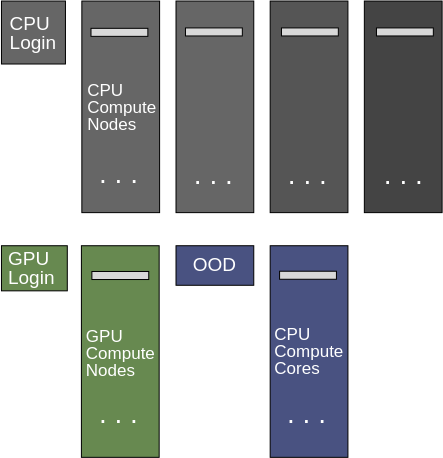
\includegraphics[keepaspectratio]{trilnodes.png}}
\end{column}

\begin{column}{0.47\linewidth}\setlength{\parskip}{0.5\baselineskip}
\small\vspace{-1mm}

\pause

\begin{block}{Login nodes}\setlength{\parskip}{0.5\baselineskip}
\phantomsection\label{login-nodes}
\vspace{-1mm}

\begin{itemize}
\tightlist
\item
  Ssh reaches the CPU or GPU login nodes.
\item
  OnDemand reaches the OOD server.
\item
  Shared among users
\item
  Meant for preparing your work and software.
\end{itemize}

\pause
\end{block}

\begin{block}{Compute nodes}\setlength{\parskip}{0.5\baselineskip}
\phantomsection\label{compute-nodes}
\vspace{-1mm}

\begin{itemize}
\tightlist
\item
  CPU: scheduled by 192-core node.
\item
  GPU: scheduled by full NVIDIA H100 GPU.
\item
  No internet access.
\item
  Read-only home directory.
\end{itemize}

\pause
\end{block}

\begin{block}{OOD compute cores}\setlength{\parskip}{0.5\baselineskip}
\phantomsection\label{ood-compute-cores}
\vspace{-1mm}

\begin{itemize}
\tightlist
\item
  Scheduled by core and memory
\item
  Internet access.
\item
  Writable home directory
\end{itemize}
\end{block}
\end{column}
\end{columns}
\end{frame}

\begin{frame}{Understanding the Trillium system}
\phantomsection\label{understanding-the-trillium-system-1}
\begin{columns}[T]
\begin{column}{0.47\linewidth}\setlength{\parskip}{0.5\baselineskip}
\vspace{-3mm}

\pandocbounded{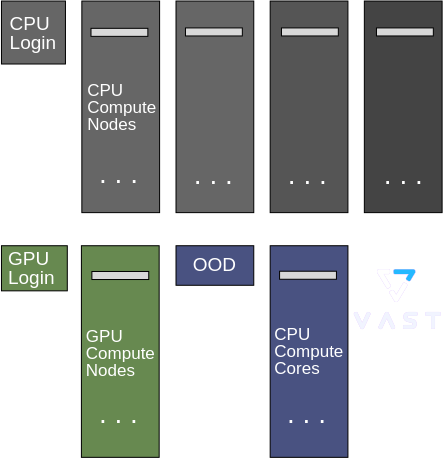
\includegraphics[keepaspectratio]{trilnodes2.png}}
\end{column}

\begin{column}{0.47\linewidth}\setlength{\parskip}{0.5\baselineskip}
\small\vspace{-1mm}

\begin{block}{Login nodes}\setlength{\parskip}{0.5\baselineskip}
\phantomsection\label{login-nodes-1}
\vspace{-1mm}

\begin{itemize}
\tightlist
\item
  Ssh reaches the CPU or GPU login nodes.
\item
  OnDemand reaches the OOD server.
\item
  Shared among users
\item
  Meant for preparing your work and software.
\end{itemize}
\end{block}

\begin{block}{Compute nodes}\setlength{\parskip}{0.5\baselineskip}
\phantomsection\label{compute-nodes-1}
\vspace{-1mm}

\begin{itemize}
\tightlist
\item
  CPU: scheduled by 192-core node.
\item
  GPU: scheduled by full NVIDIA H100 GPU.
\item
  No internet access.
\item
  Read-only home directory.
\end{itemize}
\end{block}

\begin{block}{OOD compute cores}\setlength{\parskip}{0.5\baselineskip}
\phantomsection\label{ood-compute-cores-1}
\vspace{-1mm}

\begin{itemize}
\tightlist
\item
  Scheduled by core and memory
\item
  Internet access.
\item
  Writable home directory
\end{itemize}
\end{block}
\end{column}
\end{columns}
\end{frame}

\section{Hands-on 2}\label{hands-on-2}

\begin{frame}[fragile]{Hands-on 2 (5 minutes)}
\phantomsection\label{hands-on-2-5-minutes}
\begin{itemize}
\item
  From a CPU login node, copy the python code in /home/rzon/fashion.py to your own directory.
\item
  Try to run it with \texttt{python\ fashion.py}; it should fail.
\item
  Try \texttt{pip\ install\ torch}. What does it do? Does it work after that?
\end{itemize}

Why not?
\end{frame}

\section{Software packages}\label{software-packages}

\begin{frame}[fragile]{It's a shared system}
\phantomsection\label{its-a-shared-system}
It is impossible to simultaneously install every user's required software and software version.

\pause

\begin{block}{Almost all installed software is made available using modules}\setlength{\parskip}{0.5\baselineskip}
\phantomsection\label{almost-all-installed-software-is-made-available-using-modules}
\pause

\begin{itemize}
\item
  These set environment variables (\texttt{PATH}, etc.)

  \pause
\item
  Allows multiple, conflicting versions of a given package to be available.

  \pause
\item
  \alert{\texttt{module\ overview\ {[}MODULE{]}}} shows the available software.
\end{itemize}

\pause
\end{block}

\begin{block}{Python wheels}\setlength{\parskip}{0.5\baselineskip}
\phantomsection\label{python-wheels}
\begin{itemize}
\item
  The module system does not work well for Python packages.

  \pause
\item
  One might try to just install these using \texttt{pip}, but you would get generic, non-optimized versions.

  \pause
\item
  To support optimized version of python packages, without requiring users to compile these themselves, we have a \alert{wheelhouse} of packages that you can install into \alert{virtual environments}.

  \pause
\item
  \alert{\texttt{avail\_wheels\ {[}PACKAGE{]}}} shows the available python packages.
\end{itemize}
\end{block}
\end{frame}

\begin{frame}[fragile]{Virtual environments}
\phantomsection\label{virtual-environments}
If you ``pip installed''-ed \texttt{torch} in Hands-on 2, it did something:

\pause

\begin{itemize}
\item
  A little utility called \texttt{mii} would have found a number of versions of \texttt{pip}.\vspace{-2mm}

  \pause
\item
  If you selected one, pip would install it for that version.was tied to a specific python module.\vspace{-2mm}

  \pause
\item
  Pip installed the package in \texttt{\$HOME/.local/lib/pythonVERSION/site-packages}.
\end{itemize}

But since we did not load that python module, so \texttt{python\ fashion.py} failed.

\begin{block}{Bad solution: only load a module}\setlength{\parskip}{0.5\baselineskip}
\phantomsection\label{bad-solution-only-load-a-module}
If you do \texttt{module\ load\ python/VERSION}, it would work now.

But what if you yourself need to use different sets of packages?
\end{block}

\begin{block}{Good solution: Use a virtual environment}\setlength{\parskip}{0.5\baselineskip}
\phantomsection\label{good-solution-use-a-virtual-environment}
\vspace{-2mm}

\begin{Shaded}
\begin{Highlighting}[]
\ExtensionTok{$}\NormalTok{ module load python/3.13}
\ExtensionTok{$}\NormalTok{ virtualenv }\AttributeTok{{-}{-}no{-}download}\NormalTok{ \textasciitilde{}/.virtualenvs/myenv}
\ExtensionTok{$}\NormalTok{ source }\VariableTok{$HOME}\NormalTok{/.virtualenvs/myenv/bin/activate}
\KeywordTok{(}\ExtensionTok{myenv}\KeywordTok{)} \ExtensionTok{$}\NormalTok{ pip install }\AttributeTok{{-}{-}no{-}index}\NormalTok{ torch}
\end{Highlighting}
\end{Shaded}
\end{block}
\end{frame}

\section{Hands-on 3}\label{hands-on-3}

\begin{frame}[fragile]{Hands-on 3 (10 minutes)}
\phantomsection\label{hands-on-3-10-minutes}
\begin{itemize}
\tightlist
\item
  Create the virtual environment. You will also need the package \texttt{torchvision}, so:
\end{itemize}

\begin{Shaded}
\begin{Highlighting}[]
    \ExtensionTok{$}\NormalTok{ module load python/3.13}
    \ExtensionTok{$}\NormalTok{ virtualenv }\AttributeTok{{-}{-}no{-}download}\NormalTok{ \textasciitilde{}/.virtualenvs/myenv}
    \ExtensionTok{$}\NormalTok{ source }\VariableTok{$HOME}\NormalTok{/.virtualenvs/myenv/bin/activate}
    \KeywordTok{(}\ExtensionTok{myenv}\KeywordTok{)} \ExtensionTok{$}\NormalTok{ pip install }\AttributeTok{{-}{-}no{-}index}\NormalTok{ torch torchvision}
\end{Highlighting}
\end{Shaded}

\begin{itemize}
\item
  By the way, the options \texttt{-\/-no-downloads} and \texttt{-\/-noindex} cause this procedure to only use optimized packages from the wheelhouse.*
\item
  What pip installed in the default directory, would override the ones in the virtual environment, so remove that:
\end{itemize}

\begin{Shaded}
\begin{Highlighting}[]
    \ExtensionTok{$}\NormalTok{ rm }\AttributeTok{{-}rf} \VariableTok{$HOME}\NormalTok{/.local/lib/python}\PreprocessorTok{*}\NormalTok{/site{-}packages}
\end{Highlighting}
\end{Shaded}

\begin{itemize}
\item
  Make sure \texttt{python\ fashion.py} now starts properly.

  \pause
\item
  And see what fails next.\pause (really? sorry yeah, really.)
\end{itemize}
\end{frame}

\begin{frame}[fragile]{To the compute nodes!}
\phantomsection\label{to-the-compute-nodes}
\begin{Shaded}
\begin{Highlighting}[]
\KeywordTok{(}\ExtensionTok{myenv}\KeywordTok{)} \ExtensionTok{$}\NormalTok{ python fashion.py}
\ExtensionTok{CPU}\NormalTok{ time limit exceeded}
\end{Highlighting}
\end{Shaded}

\begin{itemize}
\item
  We ran this on a CPU login node, a \textbf{shared resource}.
\item
  For fairness, each user can only run a limit amount of time.

  \pause
\item
  For longer runs, you need to submit a job to run on the compute nodes.

  \pause
\end{itemize}

\alert{Caveat (again)! This task here is not really heavy enough to warrant using a full 192-core Trillium node!}
\end{frame}

\begin{frame}{Peculiarities of Trillium compute nodes}
\phantomsection\label{peculiarities-of-trillium-compute-nodes}
\begin{columns}[T]
\begin{column}{0.31\linewidth}\setlength{\parskip}{0.5\baselineskip}
\vspace{\baselineskip}

\begin{enumerate}
\item
  You always get a multiple of 192-core nodes (or a multiple of GPUs)

  \pause
\item
  They run batch jobs through a scheduler

  \pause
\item
  They run detached from a terminal

  \pause
\item
  Cannot write to \$HOME

  \pause
\item
  No internet access

  \pause
\end{enumerate}
\end{column}

\begin{column}{0.62\linewidth}\setlength{\parskip}{0.5\baselineskip}
So:

\begin{enumerate}
\item
  Bundle up short and small jobs (beyond today's workshop).\\
  \vspace{\baselineskip} \vspace{\baselineskip}

  \pause
\item
  Write a job script to be submitted to the scheduler. \vspace{\baselineskip}

  \pause
\item
  Fine, but we can get emails when the job starts and ends. \vspace{\baselineskip}

  \pause
\item
  Copy everything for a job to \$SCRATCH

  \pause
\item
  Write a separate python script to download the data (or run once from the login node).
\end{enumerate}
\end{column}
\end{columns}
\end{frame}

\section{Hands-on 4}\label{hands-on-4}

\begin{frame}[fragile]{Hands-on 4 (20 min)}
\phantomsection\label{hands-on-4-20-min}
\begin{itemize}
\tightlist
\item
  Setup a directory in scratch:\vspace{-1mm}
\end{itemize}

\begin{Shaded}
\begin{Highlighting}[]
    \KeywordTok{(}\ExtensionTok{myenv}\KeywordTok{)} \ExtensionTok{$}\NormalTok{ mkdir }\VariableTok{$SCRATCH}\NormalTok{/myrun}
    \KeywordTok{(}\ExtensionTok{myenv}\KeywordTok{)} \ExtensionTok{$}\NormalTok{ cp fashion.py }\VariableTok{$SCRATCH}\NormalTok{/myrun}
    \KeywordTok{(}\ExtensionTok{myenv}\KeywordTok{)} \ExtensionTok{$}\NormalTok{ cd }\VariableTok{$SCRATCH}\NormalTok{/myrun}
\end{Highlighting}
\end{Shaded}

\pause

\vspace{-3mm}

\begin{itemize}
\tightlist
\item
  Download the data from the login node:\vspace{-1mm}
\end{itemize}

\begin{Shaded}
\begin{Highlighting}[]
    \KeywordTok{(}\ExtensionTok{myenv}\KeywordTok{)} \ExtensionTok{$}\NormalTok{ python}
    \OperatorTok{\textgreater{}\textgreater{}\textgreater{}}\NormalTok{ from }\ExtensionTok{torchvision}\NormalTok{ import datasets}
    \OperatorTok{\textgreater{}\textgreater{}\textgreater{}}\NormalTok{ training\_data }\ExtensionTok{=}\NormalTok{ datasets.FashionMNIST}\ErrorTok{(}\VariableTok{root}\OperatorTok{=}\StringTok{"data"}\NormalTok{,download=True}\KeywordTok{)}
    \OperatorTok{\textgreater{}\textgreater{}\textgreater{}}\NormalTok{ exit}\KeywordTok{()}
\end{Highlighting}
\end{Shaded}

\pause

\vspace{-2mm}

\begin{columns}[T]
\begin{column}{0.47\linewidth}\setlength{\parskip}{0.5\baselineskip}
\begin{itemize}
\tightlist
\item
  Create a jobscript and submit it:
\end{itemize}

\begin{Shaded}
\begin{Highlighting}[]
    \KeywordTok{(}\ExtensionTok{myenv}\KeywordTok{)} \ExtensionTok{sbatch} \AttributeTok{{-}pdebug}\NormalTok{ jobscript}
\end{Highlighting}
\end{Shaded}
\end{column}

\begin{column}{0.47\linewidth}\setlength{\parskip}{0.5\baselineskip}
\vspace{-3mm}

\begin{Shaded}
\begin{Highlighting}[]
\CommentTok{\#!/bin/bash}
\CommentTok{\#SBATCH {-}{-}nodes=1}
\CommentTok{\#SBATCH {-}{-}ntasks=1}
\CommentTok{\#SBATCH {-}{-}cpus{-}per{-}task=192}
\CommentTok{\#SBATCH {-}{-}time=0:16:00}
\CommentTok{\#SBATCH {-}{-}mail{-}type=ALL}
\CommentTok{\#SBATCH {-}{-}mail{-}user=rzon@...}
\CommentTok{\#SBATCH {-}{-}output=jobscript\_\%j.out}
\ExtensionTok{module}\NormalTok{ load python/3.13}
\BuiltInTok{source} \VariableTok{$HOME}\NormalTok{/.virtualenvs/myenv/bin/activate}
\BuiltInTok{export} \VariableTok{OMP\_NUM\_THREADS}\OperatorTok{=}\VariableTok{$SLURM\_CPUS\_PER\_TASK}
\ExtensionTok{python} \AttributeTok{{-}u}\NormalTok{ fashion.py }
\end{Highlighting}
\end{Shaded}
\end{column}
\end{columns}
\end{frame}

\begin{frame}[fragile]{GPUs, you ask?}
\phantomsection\label{gpus-you-ask}
Yes, of course, AI workload such as this should run on GPUs.

\pause

Luckily, pytorch code can run on either a CPU or GPU dynamically.

\pause

We just have to:

\pause

\begin{columns}[T]
\begin{column}{0.47\linewidth}\setlength{\parskip}{0.5\baselineskip}
\begin{itemize}
\tightlist
\item
  log into the gpu login node
\end{itemize}

\begin{Shaded}
\begin{Highlighting}[]
    \KeywordTok{(}\ExtensionTok{myenv}\KeywordTok{)} \ExtensionTok{$}\NormalTok{ ssh trig{-}login01 }
    \ExtensionTok{$}\NormalTok{ module load python/3.13}
    \ExtensionTok{$}\NormalTok{ source }\VariableTok{$HOME}\NormalTok{/.virtualenvs/myenv/bin/activate}
    \KeywordTok{(}\ExtensionTok{myenv}\KeywordTok{)} \ExtensionTok{$}\NormalTok{ cd }\VariableTok{$SCRATCH}\NormalTok{/myrun}
\end{Highlighting}
\end{Shaded}

\pause

\begin{itemize}
\tightlist
\item
  and adapt the jobscript to ask for a GPU
\end{itemize}

\begin{Shaded}
\begin{Highlighting}[]
    \ExtensionTok{$}\NormalTok{ cp jobscript jobscriptgpu}
    \ExtensionTok{$}\NormalTok{ nano jobscriptgpu}
\end{Highlighting}
\end{Shaded}
\end{column}

\begin{column}{0.47\linewidth}\setlength{\parskip}{0.5\baselineskip}
\pause

\vspace{\baselineskip} \vspace{\baselineskip} \vspace{\baselineskip} \vspace{\baselineskip} \vspace{\baselineskip} \vspace{\baselineskip} \vspace{\baselineskip}

\begin{Shaded}
\begin{Highlighting}[]
\CommentTok{\#SBATCH {-}{-}gpus{-}per{-}node=1}
\CommentTok{\#SBATCH {-}{-}cpus{-}per{-}task=24}
\end{Highlighting}
\end{Shaded}
\end{column}
\end{columns}

\pause

\emph{Note that in jobscript, and when we ssh into another login node, the virtual environment is no longer active and modules are not loaded; you must reload and reactivate.}
\end{frame}

\section{Hands-on 5}\label{hands-on-5}

\begin{frame}{Hands-on 5 (5 min)}
\phantomsection\label{hands-on-5-5-min}
Let's run it on the GPU subcluster of Trillium!
\end{frame}

\section{Okay, but what about interactive notebooks?}\label{okay-but-what-about-interactive-notebooks}

\section{SciNet's Open OnDemand}\label{scinets-open-ondemand}

\begin{frame}{Not everything needs 192 cores, or a GPU}
\phantomsection\label{not-everything-needs-192-cores-or-a-gpu}
What if you have that one postprocessing step that you need less than 192 cores for? \vspace{\baselineskip} What if you need to do some visualization? \vspace{\baselineskip}

\pause

For interactive work of that and other kinds in python, JupyterLab is typically used.

\pause

SciNet installed the OnDemand to provide Jupyter Lab and other features in the browser.
\end{frame}

\begin{frame}{Logging into the Open OnDemand portal}
\phantomsection\label{logging-into-the-open-ondemand-portal}
\begin{columns}[T]
\begin{column}{0.47\linewidth}\setlength{\parskip}{0.5\baselineskip}
To access the Open OnDemand portal, open a web browser and navigate to the following page: \alert{\url{https://ondemand.scinet.utoronto.ca}}

\pause

You will be prompted to enter your Alliance username and password, followed by a second factor authentication via Duo or Yubikey.

\pause

Once you have logged in, you will be taken to the Open OnDemand dashboard.

\pause

From here you can access the various tools and applications available on the platform.
\end{column}

\begin{column}{0.47\linewidth}\setlength{\parskip}{0.5\baselineskip}
\pandocbounded{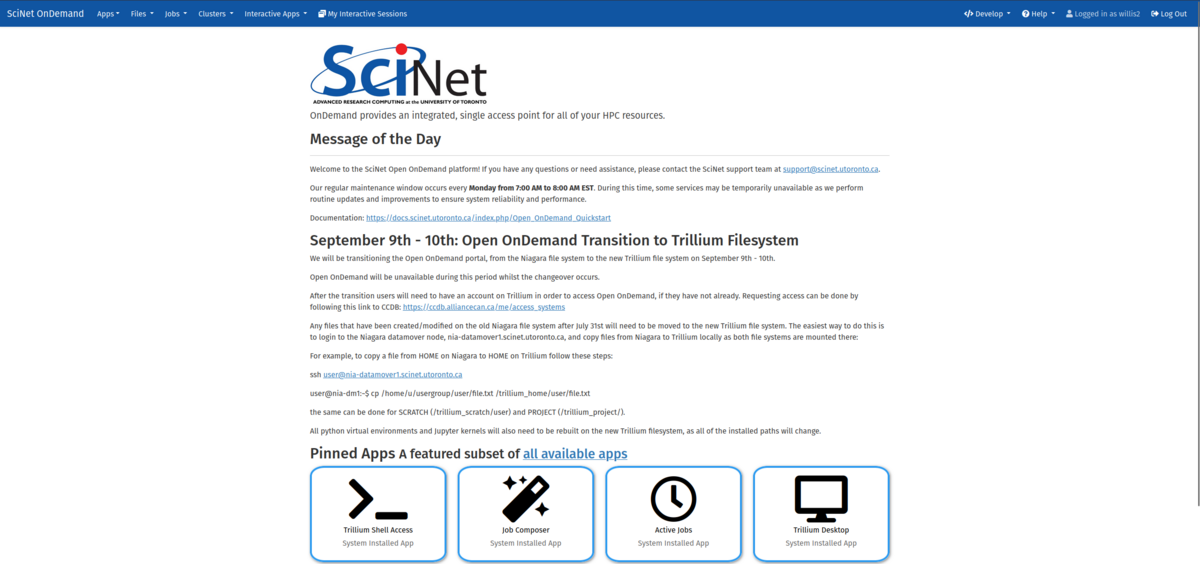
\includegraphics[keepaspectratio]{ood-dashboard.png}}
\end{column}
\end{columns}
\end{frame}

\begin{frame}[fragile]{File management}
\phantomsection\label{file-management}
The Open OnDemand platform provides a file browser.

Click on the \textbf{Files} tab and select which directory you want to manage from the drop-down (\texttt{HOME}, \texttt{SCRATCH} or \texttt{PROJECT}).

\pause

You can:

\begin{itemize}
\tightlist
\item
  Navigate through your directories
\item
  Upload/download files
\item
  Create new files/directories
\item
  Delete files/directories
\item
  Edit existing files
\end{itemize}

\pause

\emph{Note: there is a Globus button in the file browser at the top right as well, which will take you to the Globus web interface.}
\end{frame}

\begin{frame}{Interactive applications}
\phantomsection\label{interactive-applications}
Perhaps the most convenient part of Open OnDemand are its interactive applications that can be run directly from your web browser. To access the applications, navigate to the \textbf{\emph{Interactive Apps}} tab and select the application you want to run from the drop-down.

\pause

This will then bring you to the job submission page where you can choose job parameters such as:

\pause

\begin{itemize}
\tightlist
\item
  Length of job in hours
\item
  Number of cores (there are no GPUs atm)
\item
  Amount of memory to allocate (GB)
\item
  Notify me by email when the job starts
\end{itemize}

\pause

When you have chosen your job parameters click on the \textbf{\emph{Launch}} button to submit your job to the queue.

\pause

You will be taken to the \textbf{\emph{My Interactive Sessions}} page where you can see the status of your job, i.e.~queued, running or completed.

\pause

Once the job has been assigned a node and is running, you can click on the \textbf{\emph{Connect to }} button to launch the application.

\pause

The application will open in a new tab in your browser.
\end{frame}

\begin{frame}{Available applications in OnDemand}
\phantomsection\label{available-applications-in-ondemand}
\begin{itemize}
\item
  Trillium Desktop - a graphics desktop in your browser

  \pause
\item
  RStudio - an environment to run R

  \pause
\item
  VS Code - a code editor

  \pause
\item
  Paraview - a parallel visualization program

  \pause
\item
  ARM Forge - to use the parallel debugger DDT

  \pause
\item
  and last but not least: \textbf{Jupyter Lab}.
\end{itemize}
\end{frame}

\begin{frame}{Jupyter Lab}
\phantomsection\label{jupyter-lab}
We have two flavours of this:

\begin{itemize}
\item
  The default `native' Jupyter Lab
\item
  JupyterLab with Alliance software extensions. These can give you similar applications to the OOD interactive applications, but started from Jupyter.
\end{itemize}

We'll use the first here.
\end{frame}

\section{Hands-on 6}\label{hands-on-6}

\begin{frame}{Hands-on 6 (5 minutes)}
\phantomsection\label{hands-on-6-5-minutes}
Part 1: * Access OpenOnDemand * Start a Jupyter Lab session with 4 cores, 8 GB, for 1 hour. * Go to the Launcher tab.

But you won't see your `myenv' environment?
\end{frame}

\begin{frame}[fragile]{VENV2JUP}
\phantomsection\label{venv2jup}
This is an essential utility to make your virtual environments visible in the JupterHub.

In a terminal (possibly the one on OpenOnDemand):

\begin{itemize}
\item
  Load all needed modules

  \pause
\item
  Activate your environment

  \pause
\item
  And run
\end{itemize}

\begin{Shaded}
\begin{Highlighting}[]
  \KeywordTok{(}\ExtensionTok{myenv}\KeywordTok{)} \ExtensionTok{$}\NormalTok{ venv2jup}
\end{Highlighting}
\end{Shaded}

This installs some packages and puts a file in \texttt{\$HOME/.local/share/jupyter/kernels}, which is how the JupyterLab knows it exists.
\end{frame}

\section{Hands-on 7}\label{hands-on-7}

\begin{frame}[fragile]{Hands-on 7 (5 minutes)}
\phantomsection\label{hands-on-7-5-minutes}
\begin{itemize}
\tightlist
\item
  Perform the venv2jup step.
\item
  Refresh the jupyter lab interface.
\item
  Start a `myenv' notebook.
\item
  Check that it works with ``\texttt{import\ torch}'
\end{itemize}
\end{frame}

\section{Thank you for your attention!}\label{thank-you-for-your-attention}

\end{document}
